
\chapter{Method}
	
	Points within a 3d point cloud are simply represented by their x, y, z Cartesian coordinates. This means that there is a possibility that there are two points with the same x, y, z coordinates that have been acquired at different times, this is assuming that the origin is the same. Comparing these points is not as easy as one would assume, they may occupy the same point in space, but cannot simply assume that they are the same.
	
	We may get some extra data from a laser scanner, such as intensity and colour. But this doesn't really give us any information about the area surrounding these points and weather anything has changed.
	
	Situations where points need to be compared for any reason require more information than can be provided by a laser scanner. So the idea of looking at each point individually now falls away. We need to start looking at the bigger picture of what the point cloud is telling us.\\
	\\
	Machine learning is a subfield of computer science that evolved from pattern recognition and learning theory in artificial intelligence. it is in the field of machine learning that we start to look at the bigger picture of what our point clouds are telling us. Machine learning is the study of creating algorithms that can learn from and make predictions about data.\\
	\\
	The aim of this Thesis is, given an uncleaned, noisy point cloud of a room to create an .obj file with lines representing all the edges of that room.
	
	
\section{Segmentation}
	\label{segmentation-method}
	\subsection{Principal Components Analysis}
		A Principal Components Analysis (PCA) is the default method for estimating normals in Point Cloud Library. it is the fastest method because of PCL's multi-threading option for the function.
		
		A principal components analysis can be thought of as fitting an \textit{n}-dimensional ellipse to a set of data. Each axis of the ellipse represents a principal component. If an axis is large then the variance along that axis is large, and vice versa. When calculating the normal of a point set, the smallest axis is the axis with with the least variance and therefore represents the normal. This is easy to think of with a 2D disk of points, like in figure \ref{fig:PCA2D Example}. Its easy to see how the 3rd axis for these set of point will be coming out of the page, as it has to be orthogonal to the other two.
		
		\begin{figure}[H]
			\centering
			\begin{subfigure}{.5\textwidth}
				\centering
				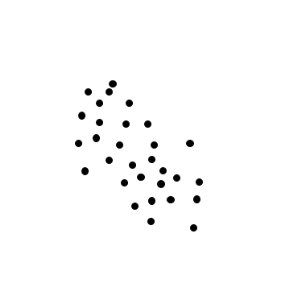
\includegraphics[width=0.6\linewidth]{Includes/images/pca1}

				\label{fig:sub1}
			\end{subfigure}%
			\begin{subfigure}{.5\textwidth}
				\centering
				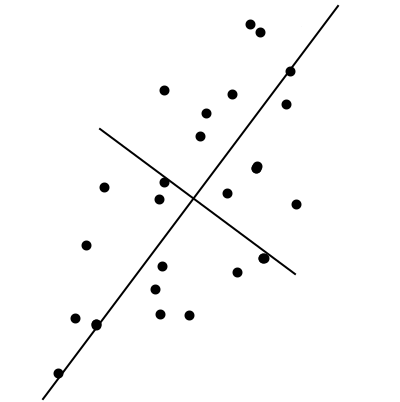
\includegraphics[width=0.6\linewidth]{Includes/images/pca2}

				\label{fig:sub2}
			\end{subfigure}
			\caption{A 2D representation of a Principal Components Analysis }
		\end{figure} 
		
		To fit this \textit{n}-dimensional ellipse we compute the covariance matrix of the data set and calculate the eigenvalues and corresponding eigenvectors of this covariance matrix.
		
		\subsubsection{Calculating the Covariance Matrix of a given set of 3D points}
			The covariance matrix, $C$, is calculated for each point $p_i$ as follows:
			
			\begin{equation}
			C = \frac{1}{k} \sum_{i=1}^{k}.(p_i - \bar{p}).(p_i - \bar{p})^T
			\end{equation}
			
			Where $k$ is the number of points in the neighborhood of point $p_i$, and $\bar{p}$ is the 3D centroid of the nearest neighbors.
				
		\subsubsection{Calculating Eigenvalues and Eigenvectors}
			Eigenvalues, $\lambda_j$, and eigenvectors, $\vec{v_j}$, are calculated on the covariance matrix, $C$, for a given point:
			
			\begin{equation}
			C \vec{v_j} = \lambda_j \vec{v_j}
			\end{equation}
			After solving the system and getting results for $\lambda_j$ and $\vec{v_j}$, the smallest eigenvalue and its corresponding eigenvector is are as the normal $\vec{n_i}$ for that point.\\
			\\
			\\
			There is no mathematical method for determining the sign of the normal, its orientation as computed in the PCA is ambiguous, and not consistent over the whole point cloud. 
			
			The solution to this issue is simple. If the viewpoint is known, in the case of laser scans the scan center, then orientate all normals $\vec{n_i}$ towards the viewpoint. This whole process results in what is seen in figure \ref{fig:Normals}.
			
			\begin{figure}[H]
			\centering
			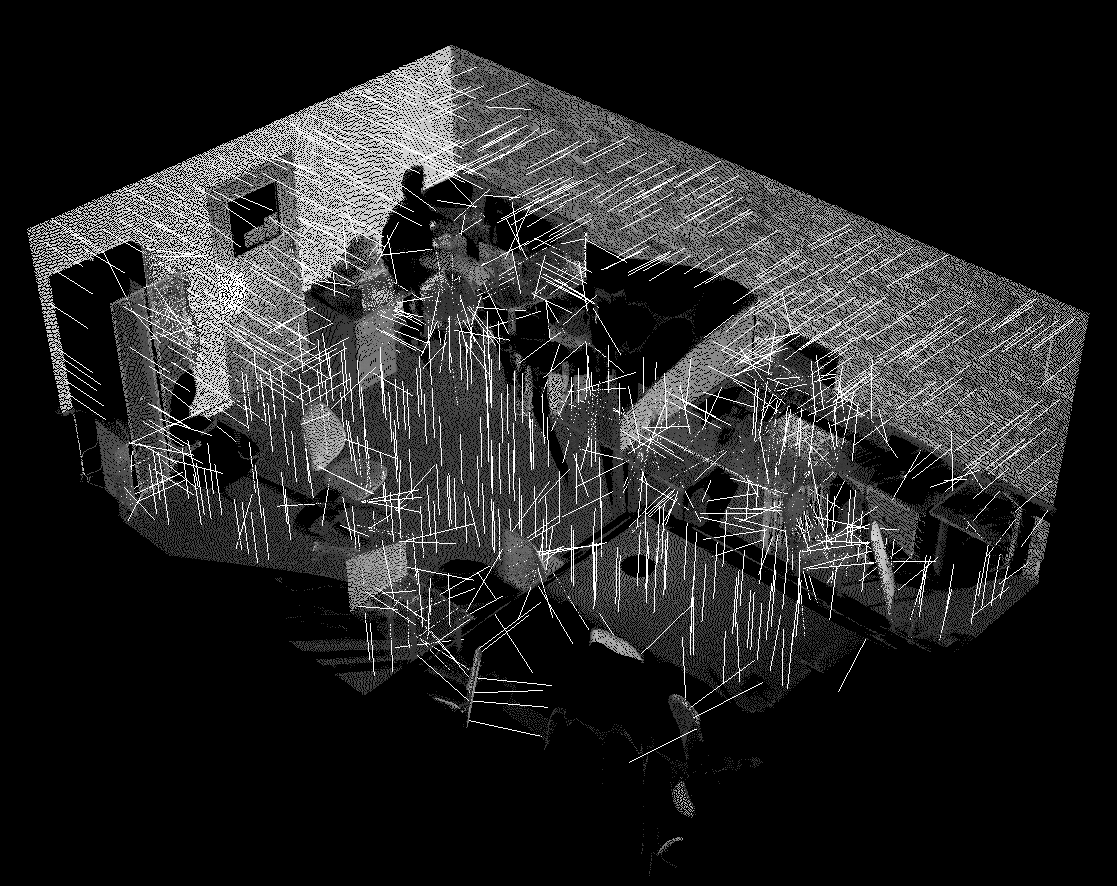
\includegraphics[width=0.7\linewidth]{Includes/images/Normals}
			\caption{Normals calculated over a cut down section of a point cloud (the roof has been removed for ease of viewing)}
			\label{fig:Normals}
			\end{figure}
		

				
	\subsection{Region Growing}
	
		
		A Region growing algorithm starts off by selecting seed points. This is done by calculating the curvature of each point then storing all the points in an array, sorted by their curvature value. The reason for this is because the point with the least curvature value is located in the flattest section of the point cloud. Now regions can begin to be grown using the flattest points in the cloud as seed points. 
		
		The first point in the sorted array is chosen as the first seed point:
		
		\begin{itemize}
			
			\item The nearest neighbors to this point are looked at and are either rejected or accepted into the region based on user defined criteria such as normal deviation and smoothness and curvature constraints.
			
			\item Once a point is accepted into the region, the process starts again based on that point.
			
			\item Once no more points are found for that particular seed, or the region reached a specified maximum, the seed is removed from the set of seeds and the region is added to the global segment list. 
			
		\end{itemize}
		
		This is repeated while the list of available points is not empty.
		
		If after a seed point has been through the process and the number of points does not reach the user defined minimum size, the region removed from the cloud as unclassified. Unclassified points are removed from the cloud completely after the process is terminated.
		
		
		\begin{figure}[H]
			\centering
			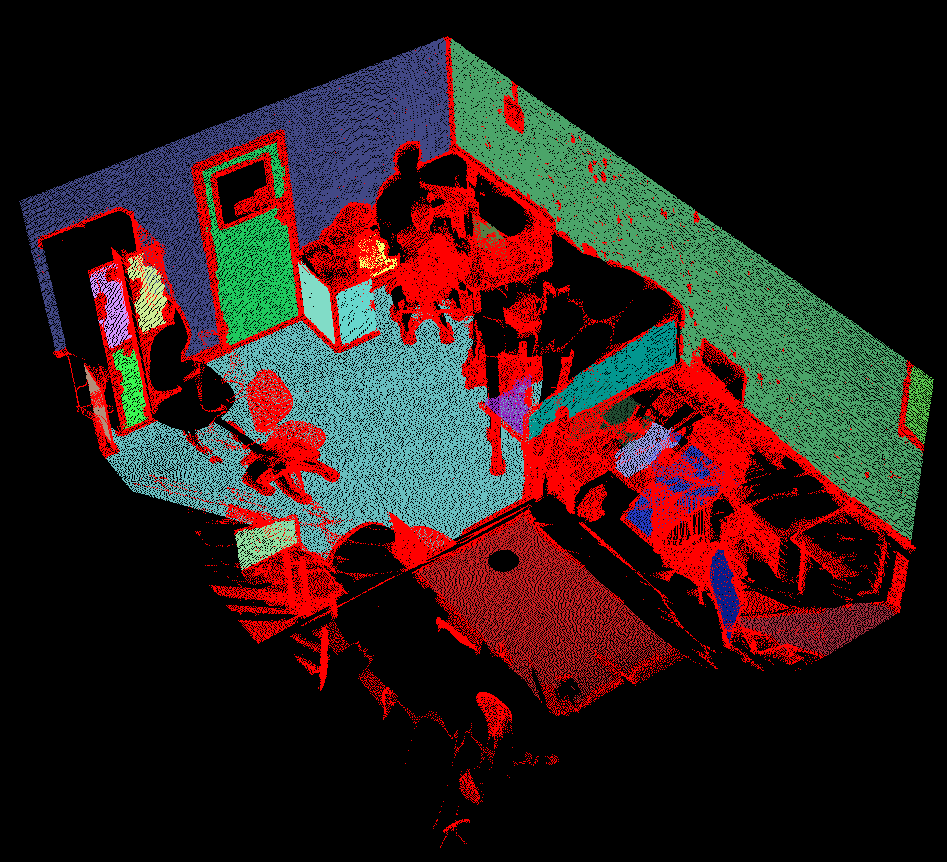
\includegraphics[width=0.5\linewidth]{Includes/images/GrownRegions}
			\caption{Red Points represent unclassified points}
			\label{fig:GrownRegions}
		\end{figure}
		
		The unclassified points are of no use, and are therefore removed.
		
		
		\begin{figure}[H]
			\centering
			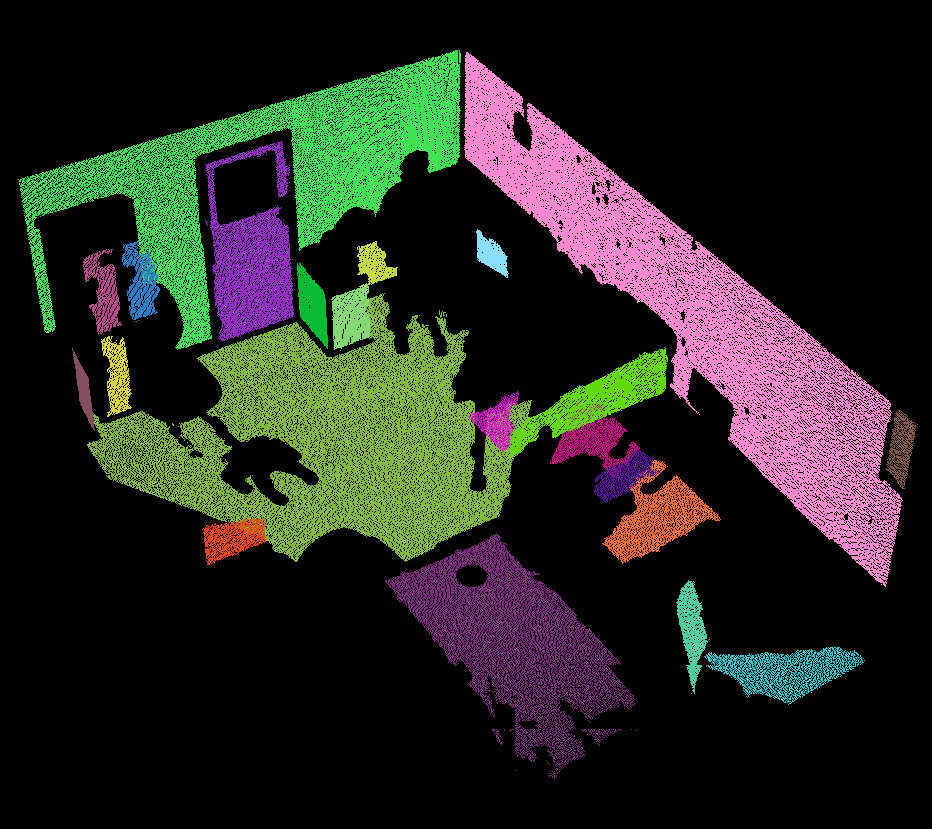
\includegraphics[width=0.5\linewidth]{Includes/images/RG-noUnclass}
			\caption{Segmented room with unclassified points removed}
			\label{fig:RG-noUnclass}
		\end{figure}
		
		The segments are coloured randomly to make them easier to distinguish for the user.
		
		A pseudo-code algorithm for region growing can be found in appendix A.
		
	
\section{Surface Extraction}
	
		\subsection{Random Sample Consensus}
		\label{RANSAC expl}
			Random Sample consensus (RANSAC) is used to estimate a normal to the segment by fitting a plane to it.
			
			RANSAC achieves this goal by iteratively selecting a random subset of the original data, this subset of the original data is considered inliers. A model is fitted and the hypothesis that this is the correct model is then tested as follows:
			
			\begin{itemize}
				\item All other data is then tested against this model, if a point fits well it is considered a hypothetical inlier.
				
				\item The model is considered a reasonably good fit if enough points are considered inliers.
				
				\item The model is then re-estimated from all hypothetical inliers, as opposed to only the initial set.
				
				\item Then finally the model is evaluated by calculating the error of all the points relative to the model.
			\end{itemize}
			
			This process is repeated a fixed number of times, each time either rejecting the model if there are too few inliers, or replacing the last saved model if the error is lower.
			
			
			\subsubsection{Choosing number of iterations in RANSAC method}
				$k$ (the number of iterations) required for a successful estimation within a certain probability can be calculated:
				
				\begin{equation}
					k = \frac{\log(1-p)}{\log(1- w^n)}
				\end{equation}
				
				Where P(success) = $p$ and P(Selecting an inlier) = $w$ and $n$ = the points that are needed to create the initially estimated model(in 3D case of plane fitting $n = 3$)\\
				\\
				$w$ is usually not known but a rough estimate can be found.\\
				\\
				Below is a 2D representation of RANSAC with a line.
			
				\begin{figure}[H]
					\centering
					\begin{subfigure}{.5\textwidth}
						\centering
						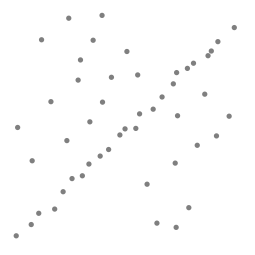
\includegraphics[width=1\linewidth]{Includes/images/random_sample_example1}
						\label{fig:RANSAC1}
					\end{subfigure}%
					\begin{subfigure}{.5\textwidth}
						\centering
						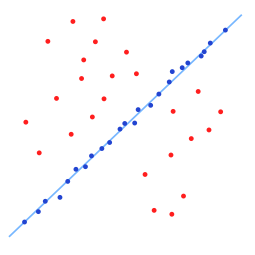
\includegraphics[width=1\linewidth]{Includes/images/random_sample_example2}
						\label{fig:RANSAC2}
					\end{subfigure}
					\caption{A 2D representation of RANSAC showing inliers in blue and outliers in red}
				\end{figure} 
			 
				
				A pseudo-code algorithm for RANSAC can be found in appendix A.
		\subsection{Segment selection}
			Segment selection is the process of filtering out useful segments and removing segments that add nothing to the final result. The process of deciding which segments to keep and which ones to remove is simple, segments are kept or rejected on the basis of 2 criteria:
			
			\begin{description}
				\item[Vertical Extent] - The  difference between the highest and lowest points in the segment
				\item[Angle from vertical] - The angle between the segment and vertical.
			\end{description}
			
			Once The filtering has taken place only big planar segments that represent the extents of the room are left.
			
		
\newpage
\section{Model Generation}
	\subsection{Bounding Box Generation}
		There are two types of Bounding boxes:
		
		\begin{figure}[H]
			\centering
			\begin{subfigure}{.5\textwidth}
				\centering
				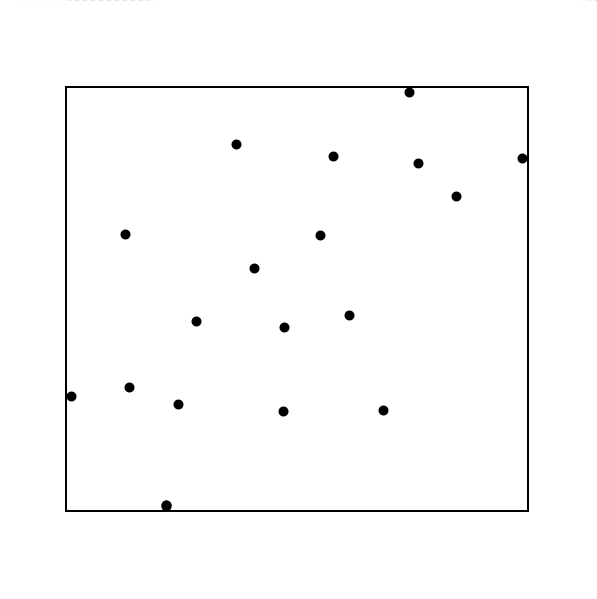
\includegraphics[width=0.7\linewidth]{Includes/images/Axis-Aligned}
				\caption{AABB}
				\label{fig:AABB}
			\end{subfigure}%
			\begin{subfigure}{.5\textwidth}
				\centering
				\includegraphics[width=0.7\linewidth]{"Includes/images/Orienrted Bounding box"}
				\caption{OBB}
				\label{fig:OBB}
			\end{subfigure}
			\caption{(a) an Axis-Aligned Bounding Box, (b) an Oriented Bounding Box}
		\end{figure}
		
		An Axis-Aligned bounding Box is a 3-dimensional box, containing all the points in a point set, aligned with the $x,y,z$ axes of the 3-dimensional Cartesian space of the point set.\\
		
		An Oriented Bounding Box is a 3-dimensional box, containing all the points in a point set, aligned with the principal components of the point set.
		
		\subsubsection{Creating an Axis Aligned Bounding Box}
			An axis Aligned Bounding Box is created through a simple maximum and minimum process.
			Extract the maximum $x,y,z$ points in the set as well as the minimum $x,y,z$ points and use them to create a box around the point set.
		
		\subsubsection{Creating an Oriented bounding Box}
			Creating an object oriented bounding box is a 6 step process.
			\begin{description}
				\item[Step 1] Compute 3D centroid and the covariance matrix of the point set
									
				\item[Step 2] Extract the eigenvectors of the covariance matrix. These eigenvectors represent the orientation of the OBB
				
				\item[Step 3] Calculate the transformation parameters between the eigenvectors and the $x,y,z$ axes.
				
				\item[Step 4] Use these parameters to transform the point set to the $x,y,z$ axes.
				
				\item[Step 5] Fit a normal AABB to the point set.
				
				\item[Step 6] Transform the point set as well as the calculated AABB back to their original positions. The AABB not becomes an oriented bounding box.
			\end{description}
			
	\subsection{Plane with Plane Intersection}
	\label{plane-planeInter}
	The fitting of planes to segments as spoken about in Section \ref{RANSAC expl} is a precursor to finding the intersection line of planar segments. Once a plane has been fitted to each segment, finding the line of intersection is simple 3D geometry.
	
	The intersection of two planes with the equations $a_1x + b_1y + c_1z = d_1$ and $a_2x + b_2y + c_2z = d_2$ will result in a parameterized line, $L$, with the form $L = L_0 + t\vec{u}$ where $\vec{u}$ is the direction vector of the line and $L_0$ is a point on the line.
	
	The direction of the line of intersection is the cross product of the two plane normals. Given:
	
	$\vec{n_1} = \begin{bmatrix}a_1\\b_1\\c_1\end{bmatrix}$  And $\vec{n_2} = \begin{bmatrix}a_2\\b_2\\c_2\end{bmatrix}$\\
	\\
	then $\vec{u}$  =  $\vec{n_1} \times \vec{n_2}  $.\\
	\\
	After calculating $\vec{u}$, to fully define the line, a specific point on it must be found.
	
	That is, we need to find the point $L_0 = (x_L,\:y_L,\:z_L)$. There are 4 methods to do this:
	\begin{enumerate}
	\item Through a direct linear equation, this method however requires a user to set either a variable to zero. This is not practical.
	
	\item By creating a third plane and intersecting the 3 planes to to get a point.
	
	\item by creating a line on one of the planes and intersecting the line with the other plane. 
	
	\item Construct system of equations using Lagrange multipliers with one objective function and two constraints. This is the method that Point cloud library uses.
	\end{enumerate}
	
	Through some derivation using Lagrange multipliers a system of equations is formed:
	
	
	\[
	\begin{bmatrix}
	2 & 0 & 0 & a_1 & a_2 \\
	0 & 2 & 0 & b_1 & b_2 \\
	0 & 0 & 2 & c_1 & c_2 \\
	a_1 & b_1 & c_1 & 0 & 0 \\
	a_2 & b_2 & c_2 & 0 & 0
	\end{bmatrix}
	b=
	\begin{bmatrix}
	0 \\
	0\\
	0 \\
	-d_1 \\
	-d_2 
	\end{bmatrix}
	\]
	
	\[
	where\: b = 	\begin{bmatrix}
		x_L \\
		y_L\\
		z_L \\
		\lambda \\
		\mu 
	\end{bmatrix}
	\]
	\newline
	\newline
	From this we have the equation of the line, $L = \begin{bmatrix}
	x_L \\
	y_L\\
	z_L 
	\end{bmatrix} + t\vec{u}$.
	
	\subsection{Orthogonal Distance of point to line}
	\label{DistanceOfPointToLine}
	The distance from a point to a line is reasonably ambiguous as it could be to any point on the line. The orthogonal distance to a line is not ambiguous. It is the shortest distance from the point to the line.
	
	\begin{figure}[H]
		\centering
		\includegraphics[width=0.7\linewidth]{"Includes/images/OrthogDist to line"}
		\caption{Orthogonal distance, $d$, to a  line}
		\label{fig:OrthogDisttoline}
	\end{figure}
	
	\noindent\cite{weisstein_point-line_????} explains it as follows:
	
	A line in 3-dimensions can be represented by 2 points, $\vec{x}_1 = (x_1,y_1,z_1)$ and $\vec{x}_2 = (x_2,y_2,z_2)$ giving:\\
	
	\begin{equation}\label{LineEqn}
	L = \begin{bmatrix}
	x_1 \\
	y_1\\
	z_1 
	\end{bmatrix} + \begin{bmatrix}
	x_2 - x_1 \\
	y_2 - y_1\\
	z_2 - z_1
	\end{bmatrix}t
	\end{equation}
	
	\noindent The squared distance from point $X_0$ and a point on the line with parameter $t$ is therefore:
	\begin{equation}\label{d^2}
	d^2 = [(x_1 - x_0) + (x_2 - x_1)t]^2 + [(y_1 - y_0) + (y_2 - y_1)t]^2  + [(x_1 - z_0) + (z_2 - z_1)t]^2 
	\end{equation}

	\noindent To minimize the distance, set $d(d^2)/dt = 0$ and solve for $t$ to obtain:
	
	\begin{equation}\label{formT}
	t = - \frac{(\vec{x_1} - \vec{x_0}) \cdot (\vec{x_2} - \vec{x_1})  }{\norm{(\vec{x_2} - \vec{x_1})}^2}
	\end{equation}
	
	The minimum distance can then be found by plugging $t$ back into equation \ref{d^2} and simplifying to obtain:
	
	\begin{equation}
	d^2 = \frac{ \norm{ (\vec{x_2} - \vec{x_1}) \times (\vec{x_1} - \vec{x_0})}^2  }{\norm{(\vec{x_2} - \vec{x_1})}^2}
	\end{equation}
	
	and taking the square root of both sides results in:
	
	\begin{equation}
	d = \frac{ \norm{ (\vec{x_0} - \vec{x_1}) \times (\vec{x_0} - \vec{x_2})}}{\norm{(\vec{x_2} - \vec{x_1})}}
	\end{equation}

	\subsection{Project points onto line}
	\label{ProjectionOntoLine}
	Projecting a point onto a line in 3-dimensional space is a similar problem to finding the orthogonal distance to a line. With the standard line equation of a line represented by two points:
	
	\begin{equation}\tag{\ref{LineEqn}}
		L = \begin{bmatrix}
		x_1 \\
		y_1\\
		z_1 
		\end{bmatrix} + \begin{bmatrix}
		x_2 - x_1 \\
		y_2 - y_1\\
		z_2 - z_1
		\end{bmatrix}t
	\end{equation}
	
	In both, projecting a point and orthogonal distance, cases you need to know a value for $t$. The formula for this, shown in equation \ref{formT}. Once $t$ has been calculated getting the projected point is as simple as substituting its value into equation \ref{LineEqn} and seeing the resulting $x,y,z$ point. This point is the orthogonal projection of the point onto the line.
	
	\subsection{Creating an OBJ file}
	
	Due to the fact that obj files are plain text they are easy to write in the same way as a text file, as long as the format is correct. Obj files support many different types, these types are all differentiated by using a keyword at the beginning of each line. 
	
	For example writing a 3 planar objects that make a small portion of a cube will result in an obj file that looks as follows:
	\newpage
	\begin{lstlisting}
	#Vertex List
	v 0 0 0
	v 1 0 0
	v 1 1 0
	v 0 1 0
	v 1 0 1
	v 0 0 1
	v 0 1 1

	#face list
	o object.side.1
	f 1 2 3 4
	o object.side.2
	f 1 2 5 6
	o object.side.3
	f 1 6 7 4
	\end{lstlisting}
	And results in a model that looks like this:
	
	
	\begin{figure}[H]
		\centering
		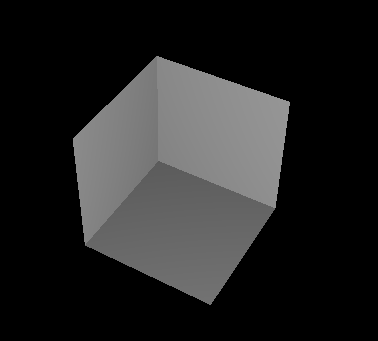
\includegraphics[width=0.5\linewidth]{Includes/images/half-box}
		\caption{3 sides of a cube}
		\label{fig:half-box}
	\end{figure}
	
	It is also possible to save textures and colours in an obj file by creating a .mtl (material) file. In the material file colours are defined in a similar way to obj files with "ka" representing an ambient colour "kd" a diffuse colour and "ks" a specular colour. 
	
	A material file also offers the ability to use texture maps, which are essentially maps of what colour is where for specific objects. Texture maps are stored in a .tga file.
	
	
		

	


